\chapter{MAPA-CSMA协议设计}
MAPA-CSMA(Mobile-node Accssibility and Playload Adaptivity based CSMA)协议是根据水声网络数据采集的需求,针对有移动节点接入的单跳网络场景设计的协议。协议的基本流程参照了802.11协议,基于带有RTS/CTS模式的CSMA/CA机制,同时采用二进制退避算法计算随机退避的时间。在此基础上,考虑到移动节点的接入,加入了BCT包来通知固定节点开始发送数据。同时,随着网络负载的增加,RTS/CTS握手带来的竞争开销较大。因此,根据负载情况的不同,可以采取不同的数据包传输流程,即在较大网络负载时,一次RTS/CTS握手后发送节点传输两个数据包,目标节点在接收到第二个数据包后再进行ACK应答。

\section {基本原理介绍}
\subsection{RTS/CTS模式}
RTS/CTS模式是通过控制包预约信道来减少数据包碰撞,即用短包的碰撞代替长数据包的碰撞。发送节点准备发送数据时,首先侦听DIFS时间,如果信道空闲则开始发送RTS帧预约信道。RTS帧中包括了源节点地址,目标节点地址和本次通讯需要的最大持续时间。目标节点接收到RTS后,侦听SIFS时间后发送CTS帧进行响应。CTS帧中同样包括了源节点地址,目标节点地址和本次通讯需要的最大持续时间。非目标节点的其他节点在接收到RTS、CTS帧后,按照最大持续时间设置NAV(Network Allocation Vector 网络分配矢量),进行退避。源节点接收到CTS后,侦听SIFS时间后发送DATA帧。目标节点接收到数据包后,侦听SIFS时间后发送ACK包响应。其他节点接收到ACK包后停止退避。
\begin{figure}[ht]
	\centering
	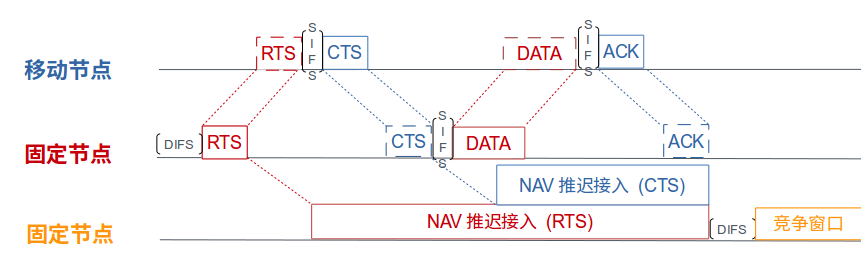
\includegraphics[scale=0.4]{figures/rtscts.png}
	\caption{
		RTS/CTS工作模式
	}
	\label{fig:example}
\end{figure}
\subsection{二进制退避算法}
具体算法描述如下:当一个节点要向信道发送数据时,首先侦听信道状态,若信道空闲且空闲时间达到一个DIFS时,节点立即进行数据发送,否则,即节点侦听到信道状态为“忙“,此时节点会一直侦听下去,直至侦听到节点空闲一段DIFS时间后,根据退避算法产生一个退避时间值存入退避计时器,如果此时退避计时器里面已经有了退避时间值,那么就不将新产生的退避时间值存入退避计时器,然后进行退避,以避免和其它节点发生冲突。退避时间值是退避时隙(Slot Time)的整数倍,退避时隙(Slot Time)是按物理层特性产生的值。节点在选好退避时间值后,如果信道在其退避期间一直空闲,那么节点会在一个完整的退避时隙后将退避时隙数减1,如果信道一直空闲到退避时隙数减到O时,那么节点就发送数据,否则,即退避过程中又侦听到“忙”,则进行冻结退避计时器,停止退避,直至再次侦听到一段DIFS时间信道空闲后,再次启动退避计数器进行退避(退避时间值从上次退避后的值开始计算)。
\begin{figure}[ht]
	\centering
	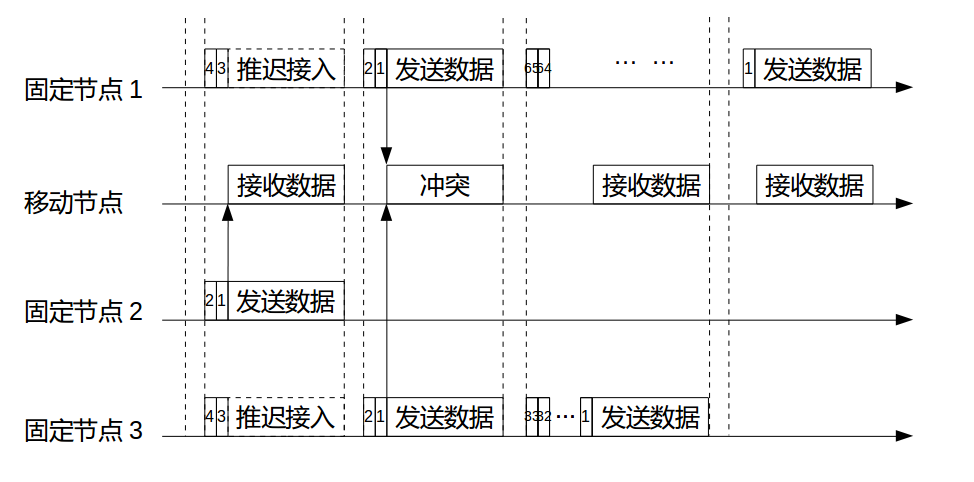
\includegraphics[scale=0.4]{figures/backoff.png}
	\caption{
		RTS/CTS工作模式
	}
	\label{fig:example}
\end{figure}
\subsection{时隙和帧间间隔}
时隙(SlotTime)是指的一个时间片段,节点竞争接入信道之前需要经过相应的随机退避过程,退避过程就是由很多个时隙所组成的。参考802.11协议,时隙定义为
\begin{equation}
\begin{aligned}
SlotTime=&CCATime\mbox{(信道监测时间)}+RxTxTurnaroundTim\mbox{(发送接收)}\\&\mbox{(转换时间)}+PropagationTime\mbox{(传播延迟)}+MACProcessing\\&Delay\mbox{(MAC层处理延迟)}
\end{aligned}
\end{equation}

短帧间间隔SIFS(Short Interfram Space)是最短的时间区段,用来间隔一次对话中的帧,如响应帧(CTS/ACK)和相邻的DATA帧等。在帧交换的两次传输之间使用最短间隔,可以防止其它正在等待信道的节点试图使用信道。参考802.11协议,SIFS定义为
\begin{equation}
\begin{aligned}
SIFSTime=&RXRFDelay\mbox{(射频延迟)}+RXPLCPDelay\mbox{(物理层头部接收)}\\&\mbox{(延迟)}+MACProcessingDelay\mbox{(MAC层处理延迟)}+ RxTx\\&TurnaroundTime\mbox{(发送接收转换时间)}
\end{aligned}
\end{equation}

分布协调功能帧间间隔DIFS(DCF Interframe Space)用于节点开始发送数据之前监测信道否空闲。如果信道已经空闲,则节点仍需等待DIFS段时间才开始发送数据;而如果在DIFS时间段内任一时刻信道被监测为忙,则节点不得不推迟它的数据发送。DIFS定义为
\begin{equation}
DIFS=SIFS+(2*SlotTime)
\end{equation}

在水声信道环境中,由于传播时延导致时隙时间过长,进而导致DIFS和随机退避时间过长,即数据传输时空闲时间过长,影响了协议的整体性能。减小时隙时间可以减小空闲时间占比,但同时也会带来包冲突概率的增加。综合这两方面的影响,最后将时隙时间设定为0.5s,SIFS设定为0.5s。
\section {移动节点接入离开机制}
通过引入BCT包控制移动节点的接入和离开,其中包括了源节点地址,目标节点地址和网络负载情况。移动节点以$\frac{1}{T_{interval}}$速率定时发送广播包BCT,开始向最近的移动节点发送CBR数据流。如果固定节点在$2*T_{interval}$时间内没有接收到广播包,则停止发送CBR数据流。
\begin{figure}[!ht]
	\centering
	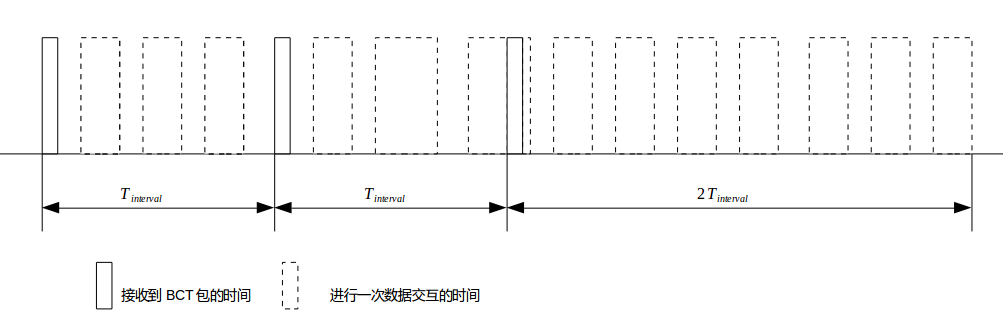
\includegraphics[scale=0.4]{figures/mj.png}
	\caption{
		移动节点接入离开机制
	}
	\label{fig:example}
\end{figure}
BCT包的发送接收不影响正在进行的一轮传输。例如在发送节点接收到CTS还未发送DATA包时接收到了BCT包,发送节点的状态仍为MAC\_CTS,在接收完BCT包后,继续发送DATA包。

HASH表

\section {数据包重传机制}
考虑到减小时隙时间导致载波侦听时间不够充分,包冲突概率增加,以及BCT包的引入带来的包冲突可能性这两个方面,加入了数据包重传机制。在802.11协议中,源节点发送了DATA包但没有收到ACK确认包的情况下,会在发送函数定时器超时后重新开始一轮新的数据传输,经过退避时间和DIFS时间倒计时后再发送RTS。这个重传流程在包冲突概率较大的情况下开销过大,影响传输性能。

因此,在发送DATA包超时后立即重传DATA包是一个可行的解决方法。同时,需要修改其他节点的推迟接入时间,在原推迟时间的基础上加上timeout(DATA包一次发送超时时间)、SIFS、txtime(传输时间)和MaxPropagationDelay(最大传播时延)。

\begin{figure}[!ht]
	\centering
	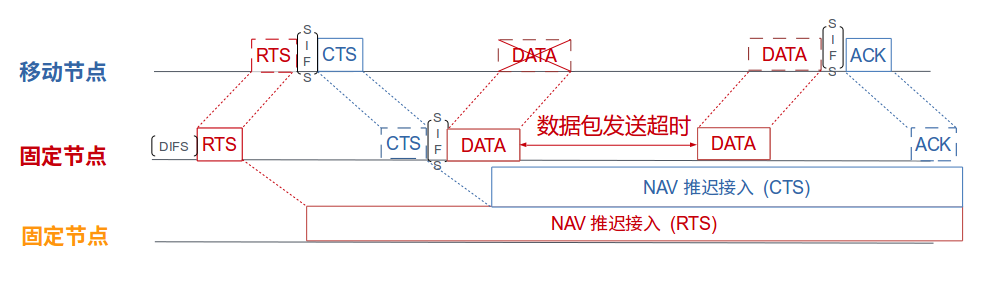
\includegraphics[scale=0.4]{figures/chongchuan.png}
	\caption{
	     数据包一次传输超时情况下的数据包重传流程
	}
	\label{fig:example}
\end{figure}

\section {基于负载变化的数据包发送机制}
网络负载较大时,数据包的RTS/CTS握手机制带来的控制开销较大,对于不同的网络负载情形,可以采用不同的数据包传输机制。在高负载的情况下,发送节点可以在一次RTS/CTS握手后发送两个DATA包,两个DATA包间间隔SIFS,接收节点在接收到第二个DATA包后发送ACK信号。低负载的情况下,仍然采用原来的流程。

由于数据包传输机制的改变,节点的推迟接入时间和发送超时时间会有不同。可以通过在BCT包中增加一位数据位标志网络的负载情况,固定节点在接收到BCT广播后更改自己的数据传输模式。
\begin{figure}[ht]
	\centering
	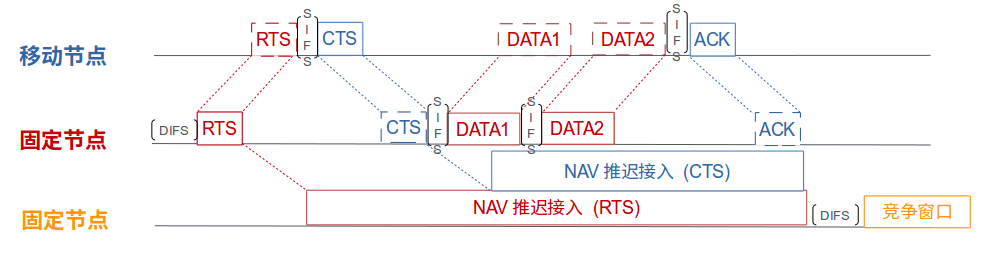
\includegraphics[scale=0.4]{figures/highload.png}
	\caption{
		高负载情况下的数据传输流程
	}
	\label{fig:example}
\end{figure}



\endinput